% ============================================================
% ConsistXApp
% Revised manuscript
% Target journal: Annals of Telecommunications (sn-jnl.cls)
% ============================================================

\documentclass[pdflatex,sn-mathphys-num,iicol,oneside]{sn-jnl}

% ============================================================
% Packages
% ============================================================

\usepackage{amsmath}
\usepackage{amssymb}
\usepackage{bm}
\usepackage{booktabs}
\usepackage{array}
\usepackage{tikz}
\usepackage{url}
\usepackage{xurl}
\usepackage{graphicx}
\usepackage{float}
\usepackage{microtype}
\usepackage{xspace}
\usepackage{enumitem}

\usetikzlibrary{
  arrows.meta,
  positioning,
  fit,
  shapes.geometric
}

% ============================================================
% Algorithms
% ============================================================

\floatstyle{ruled}
\newfloat{algorithm}{t}{loa}
\floatname{algorithm}{Algorithm}

\newcommand{\algin}[1]{\textbf{Input:} #1\par}
\newcommand{\algout}[1]{%
  \textbf{Output:} #1\par
  \vspace{2pt}\hrule\vspace{3pt}%
}

\newenvironment{algsteps}
  {\begin{enumerate}[
      leftmargin=1.8em,
      itemsep=1pt,
      parsep=0pt,
      topsep=2pt,
      label=\arabic*:
    ]}
  {\end{enumerate}}

% ============================================================
% Commands and theorem environments
% ============================================================

\newcommand{\method}{\textsc{ConsistXApp}\xspace}
\newcommand{\gac}{\textsc{GAC}\xspace}
\newcommand{\cpsat}{\textsc{CP-SAT}\xspace}

\newtheorem{proposition}{Proposition}
\newtheorem{definition}{Definition}
\newtheorem{remark}{Remark}

\raggedbottom

% ============================================================
% Document
% ============================================================

\begin{document}

\title[Consistency-Guided xApp Coordination]{
Consistency-Guided xApp Coordination in the Near-RT RIC with Incremental Repair and Independent Verification
}

\author*[1]{\fnm{Lillia} \sur{Ouali}}
\email{lillia.ouali@univ-bejaia.dz}

\author[2]{\fnm{Madani} \sur{Bezoui}}
\email{mbezoui@cesi.fr}

\author[1]{\fnm{Kamal} \sur{Amroun}}
\email{kamal.amroun@univ-bejaia.dz}

\author[3]{\fnm{Ahcene} \sur{Bounceur}}
\email{abounceur@sharjah.ac.ae}

\affil*[1]{
  \orgdiv{Department of Computer Science},
  \orgname{University of Bejaia},
  \orgaddress{
    \city{Bejaia},
    \country{Algeria}
  }
}

\affil[2]{
  \orgdiv{LINEACT},
  \orgname{CESI},
  \orgaddress{
    \city{Nancy},
    \country{France}
  }
}

\affil[3]{
  \orgname{University of Sharjah},
  \orgaddress{
    \city{Sharjah},
    \country{United Arab Emirates}
  }
}

% ============================================================
% Abstract
% ============================================================

\abstract{
Independently developed xApps may issue concurrent control requests
that are mutually incompatible or violate registered service-level
constraints. We model multi-xApp arbitration as a dynamic
finite-domain constraint problem and propose \method, a pipeline
that incrementally maintains generalized arc consistency,
repairs invalid candidates by solving an expanding local subproblem,
and forwards an action only after an independently implemented
verifier has checked every hard constraint.
Repair-core expansion is directed by propagation explanations, solver
infeasibility cores, or a graph frontier. The verifier
was evaluated with zero observed divergence across four validation gates on generated test inputs.

On 250 generated static instances from five O-RAN conflict scenarios,
the verifier accepted a hard-constraint-feasible outcome in all cases.
In this exploratory multi-worker static campaign, median computational
latency was 1.8~ms for \method and 2.8~ms for complete \cpsat; the
sub-millisecond paired difference was statistically significant but
operationally modest.

The principal benefit observed in this study is amortized. Under small
sequential changes (2\% relation updates), repairing the previous verified decision
required median per-epoch latencies of 0.05--4.9~ms for 100--1{,}000 variables, compared with
2.8--25.6~ms for rebuilding and re-solving the complete model.
At $n=1000$ with 2\% relation changes, incremental-repair latency approached re-solve latency near the pooled p95 and exceeded it at the descriptive pooled p99. Furthermore, the pipeline offered no
cold-start advantage over complete \cpsat.
All guarantees are relative to the registered constraint model and do not establish physical-RAN safety.
}

\keywords{
O-RAN,
xApp conflict management,
dynamic constraint satisfaction,
generalized arc consistency,
explanation-based repair,
constraint programming,
near-real-time RIC
}

\maketitle

% ============================================================
\section{Introduction}
\label{sec:introduction}
% ============================================================

The Open Radio Access Network (O-RAN) architecture disaggregates the
radio access network and exposes its control through programmable
components. Its near-real-time RAN Intelligent Controller (Near-RT
RIC) hosts xApps, namely third-party applications that subscribe to
measurements and issue control requests through the E2 interface
within control loops ranging from tens of milliseconds to one second
\cite{polese2023oran}. Because xApps may be developed independently,
often by different vendors, they may request incompatible values of
the same parameter, steer distinct parameters toward jointly
incompatible operating points, or collectively violate a
service-level agreement (SLA). The O-RAN Alliance therefore assigns a
conflict-mitigation function to the Near-RT RIC
\cite{oran2024conflict}. The associated literature commonly
distinguishes direct, indirect, and implicit conflicts and proposes
mechanisms for their detection and resolution
\cite{adamczyk2023conflict,wadud2024qacm}.

Most existing mechanisms primarily address what a candidate action
may do to the network through profiling, digital twins, learning, or
bargaining. This paper addresses the complementary arbitration
problem that arises after finite candidate domains and conflict
relations have been registered: how should a controller construct a
joint action so that no decision violating a registered hard
constraint is forwarded, and how can the resulting intervention be
audited?

We answer with \method, a coordination pipeline that combines three
established constraint-programming mechanisms in an O-RAN control
architecture. First, an incremental generalized arc-consistency
(\gac) stage removes values having no support in an incident hard
relation, reuses propagation state across decision epochs, and
restores affected values when a relation is relaxed. Second, when a
decoded candidate violates one or more relations, a solver-based
repair stage solves an induced subproblem. The violated constraints
seed a variable core, variables outside the core are fixed to the
candidate values, and the core expands according to propagation
explanations, solver infeasibility cores, or a deterministic frontier.
The repair may escalate to the complete model. Third, an independently
implemented verifier gates every forwarded action. The architecture is
deliberately conservative: optimizer output is treated as a proposal
until it has been checked against the current registered model.

A modern constraint solver is a demanding baseline for this design.
On the small static instances used in our scenario suite, rebuilding
and solving the complete \cpsat model requires less than 3~ms in the
median. Consequently, the approximately 1~ms median difference in
favour of \method on this suite is not, by itself, a compelling reason
to deploy an additional coordination layer. The intended operating
regime is sequential: consecutive decision epochs are expected to
share most of their variables, domains, and relations.

In the evaluated implementation, rebuilding a \cpsat model at every
epoch incurs model-construction and full-model search costs that scale
with the complete generated instance. Supplying the previous solution
as a hint did not materially reduce these costs on the tested
feasibility workloads. In contrast, repairing the previous verified
decision operated on the relations invalidated by the update and on
the repair core induced by them. This comparison concerns the
evaluated Python rebuild-and-resolve implementation; it does not
establish that solution hints or other persistent incremental solvers
are ineffective in general.

The contributions of this paper are as follows.

First, we formulate registered multi-xApp arbitration as a dynamic
finite-domain constraint problem with context-dependent hard
relations, soft utility, and temporal-stability costs.

Second, we design an incremental \gac layer with restoration after
relaxing updates. We prove that filtering preserves every globally
feasible assignment and give a symmetric counterexample showing why
local consistency cannot guarantee the validity of a per-variable
decode.

Third, we introduce an explanation-guided, solver-based repair
procedure with monotone core expansion and conditional completeness.
Expanding cores resolved all 248 evaluated repair candidates, whereas fixed violated-scope repair failed on 21 of them; this success-rate difference is statistically significant under the exact paired test. We also evaluate
stronger conflict-aware decoders and show that they reduce, but do not
eliminate, the need for verified repair.

Fourth, we implement an independent forwarding verifier and evaluate
it through exhaustive comparison with an oracle, a second
implementation, property-based testing, and oracle-labelled input
mutation. These tests increase confidence in the implementation but
do not constitute a proof of verifier correctness outside the tested
input distributions.

Finally, we characterize the regime observed in the experiments:
there is no cold-start advantage over complete \cpsat up to 1{,}000
variables; sequential repair provides a growing median advantage when
updates are small; the available sample supports only descriptive
tail conclusions; local repair has a measurable objective-quality
cost; and an evaluated continuous-relaxation stage is
counterproductive.

Section~\ref{sec:background} reviews related work.
Section~\ref{sec:model} defines the coordination model.
Section~\ref{sec:method} presents \method, and
Section~\ref{sec:analysis} gives its formal properties.
Sections~\ref{sec:experiments} and~\ref{sec:results} describe the
experimental setup and results.
Section~\ref{sec:limitations} discusses threats to validity, and
Section~\ref{sec:conclusion} concludes the paper.

% ============================================================
\section{Background and Related Work}
\label{sec:background}
% ============================================================

The Near-RT RIC supports control loops between tens of milliseconds
and one second. xApps subscribe to key performance measurements
(KPMs), process network context, and issue E2 control requests
\cite{polese2023oran}. Experimental platforms such as ColO-RAN,
OpenRAN Gym, and FlexRIC support development and closed-loop
evaluation of O-RAN controllers
\cite{polese2022coloran,bonati2023openrangym,schmidt2021flexric}.

Three conflict classes are commonly distinguished
\cite{adamczyk2023conflict}. A \emph{direct conflict} occurs when two
xApps request incompatible values of the same controlled parameter.
An \emph{indirect conflict} occurs when different controlled
parameters influence a shared KPM. An \emph{implicit conflict}
couples distinct parameters and KPMs through network dynamics. Direct
conflicts can often be checked syntactically. Indirect and implicit
conflicts require a registered parameter--KPM dependency model, a
validated profile, a simulator, or a conservative operator rule.

Existing proposals include a conflict-mitigation framework integrated
into the RIC \cite{adamczyk2023conflict}, QoS-aware optimization that
maximizes the number of satisfied xApp requirements
\cite{wadud2024qacm,annals2024}, cooperative bargaining
\cite{wadud2023game}, pre-deployment profiling with statistical models
and hierarchical graphs \cite{prever2025pacifista},
digital-twin-based impact evaluation \cite{giannopoulos2025comix}, and
rule-based mitigation for mobility--energy interactions
\cite{wadud2025mobility}. XAI4C applies explainable-AI techniques to
conflict detection and mitigation \cite{varshney2025xai4c}. Its
explanations are post-hoc attributions of a learned mechanism,
whereas the explanations considered here are logical premises
replayable against a registered finite-domain model.

On the constraint-programming side, propagation removes domain values
that cannot participate in any locally supported tuple. For
non-binary relations, this property is generalized arc consistency,
which can be enforced efficiently for positive table constraints by
simple tabular reduction and related algorithms
\cite{yap2020gac,lecoutre2011str2}. Local consistency is not a
decision procedure: a \gac network may still be globally infeasible.
It can nevertheless detect some contradictions and reduce the search
space passed to a complete solver.

Dynamic constraint satisfaction studies sequences of related
problems and the incremental maintenance of consistency
\cite{bessiere1991dynamic}. Explanation mechanisms record the causes
of value removals and contradictions and support diagnosis and
repair \cite{gupta2021explanations}. Dynamic backtracking
similarly preserves useful information while revising inconsistent
decisions \cite{ginsberg1993dynamic}. Large-neighbourhood search restricts a
complete solver to a neighbourhood of a current assignment and
modifies that neighbourhood as search proceeds
\cite{shaw1998lns}. Assumption-based infeasibility analysis identifies
a sufficient subset of active assumptions causing inconsistency; such
sets need not be cardinality-minimal.

Modern solvers such as OR-Tools \cpsat combine presolve, propagation,
clause learning, integer reasoning, and optimization
\cite{perron2023cpsat,ortools}. \method does not claim to invent
incremental consistency, explanations, assumption cores, or
neighbourhood repair. Its contribution is their integration with an
independently validated forwarding gate in registered xApp
arbitration, together with an evaluation that identifies the
sequential regime in which the integration was beneficial.

% ============================================================
\section{System Model}
\label{sec:model}
% ============================================================

\subsection{Epochs, actions, and registered relations}

The Near-RT RIC operates over decision epochs
$t=1,\ldots,T$. At epoch $t$, each active action variable
$i\in\mathcal{A}_t$ has a finite base domain
\begin{equation}
D_i^t=
\left\{
a_{i,1}^t,\ldots,a_{i,d_i}^t
\right\}.
\end{equation}
A value may encode acceptance or rejection of a request, a target
cell, an execution slot, a discrete power level, a handover offset, a
resource-allocation profile, or a registered no-operation. The
coordinated action is $x_i^t\in D_i^t$. The time index is omitted when
a single epoch is considered.

A constraint $c\in\mathcal{C}_t$ has a scope
$S_c\subseteq\mathcal{A}_t$ and an allowed relation
\begin{equation}
R_c(\bm{s}_t)
\subseteq
\prod_{i\in S_c}D_i^t,
\label{eq:relation}
\end{equation}
where $\bm{s}_t$ denotes the registered context. An assignment
$\bm{x}^t$ satisfies $c$ when
\begin{equation}
\bm{x}_{S_c}^t\in R_c(\bm{s}_t).
\end{equation}

Relations may be binary or higher-order and may be derived from
operator policies, ownership rules, SLA thresholds, validated xApp
profiles, simulators, digital twins, or conservative safety rules.
Hard constraints must be satisfied before forwarding. Soft
constraints contribute only to utility.

Let
$\mathcal{C}_{t,\mathrm{hard}}\subseteq\mathcal{C}_t$
denote the hard constraints. The registered hard model is
\begin{equation}
\mathcal{M}_t=
\left(
\mathcal{A}_t,
\bm{D}_t,
\mathcal{C}_{t,\mathrm{hard}},
\bm{s}_t,
\nu_t
\right),
\label{eq:model}
\end{equation}
where $\nu_t$ is a model-version identifier. A verification result is
valid only for the model version against which it was obtained. A
production implementation must therefore bind the decision,
certificate, and forwarding event to the same version and re-verify a
candidate if the registered model changes before forwarding.

Between epochs, xApps may activate or deactivate, domains and
constraints may change, relations may tighten or relax, and SLA
thresholds may move. The modified elements form a change set
$\Delta_t$. Restrictive and relaxing changes must be distinguished.
After a restriction, previous support information may remain useful.
After a relaxation, a previously removed value may have regained
support and must be reconsidered.

\subsection{Utility and temporal stability}

Let $u_i(a_i,\bm{s}_t)$ be the utility of choosing action $a_i$ for
variable $i$, with weight $\omega_i\geq 0$. Let $v_q\geq 0$ be a soft
violation with weight $\lambda_q\geq 0$. The static utility is
\begin{equation}
U(\bm{x},\bm{s}_t)
=
\sum_{i\in\mathcal{A}_t}
\omega_i u_i(x_i,\bm{s}_t)
-
\sum_{q\in\mathcal{Q}_t}
\lambda_q v_q(\bm{x},\bm{s}_t).
\label{eq:static-utility}
\end{equation}

Given the previous verified decision $\bm{x}^{t-1}$ and
reconfiguration costs $\kappa_i\geq 0$, the weighted action churn is
\begin{equation}
H(\bm{x}^{t},\bm{x}^{t-1})
=
\sum_{i\in\mathcal{A}_t\cap\mathcal{A}_{t-1}}
\kappa_i
\mathbf{1}
\left[
x_i^t\neq x_i^{t-1}
\right].
\label{eq:churn}
\end{equation}

The general scalarized coordination problem is
\begin{align}
\max_{\bm{x}^{t}}\quad&
U(\bm{x}^{t},\bm{s}_t)
-
\mu H(\bm{x}^{t},\bm{x}^{t-1})
\label{eq:problem-objective}\\
\text{s.t.}\quad&
x_i^t\in D_i^t,
&& i\in\mathcal{A}_t,
\nonumber\\
&
\bm{x}_{S_c}^t\in R_c(\bm{s}_t),
&& c\in\mathcal{C}_{t,\mathrm{hard}},
\label{eq:problem-hard}
\end{align}
where $\mu\geq 0$ controls the preference for temporal stability. In this formulation, utility can compensate for additional churn depending on $\mu$.
However, the operational pipeline proposed in this paper implements a strictly lexicographic repair policy (Section~\ref{sec:repair}) where no utility improvement can compensate for any increase in primary churn. The complete-objective baseline evaluated in Section~\ref{sec:objective-quality} optimizes the lexicographic formulation
using the complete \cpsat model directly on the raw state. Dwell-time and cooldown rules are represented as hard relations when
their violation is not permitted.

\begin{table}[t]
\centering
\caption{Principal notation used throughout the paper.}
\label{tab:notation}
\footnotesize
\begin{tabular}{ll}
\toprule
Symbol & Meaning\\
\midrule
$t$, $T$ & Decision epoch index and horizon\\
$\mathcal{A}_t$ & Active action variables at epoch $t$\\
$D_i^t$, $d_i$ & Finite base domain of variable $i$ and its size\\
$x_i^t$, $\bm{x}^t$ & Coordinated action value and joint assignment\\
$\mathcal{C}_t$, $\mathcal{C}_{t,\mathrm{hard}}$ & Constraints and hard constraints\\
$c$, $S_c$, $R_c(\bm{s}_t)$ & Constraint, its scope, its allowed relation\\
$\bm{s}_t$ & Registered context\\
$\mathcal{M}_t$, $\nu_t$ & Registered hard model and its version identifier\\
$\Delta_t$ & Change set between epochs $t-1$ and $t$\\
$u_i$, $\omega_i$ & Per-variable utility and its weight\\
$v_q$, $\lambda_q$, $\mathcal{Q}_t$ & Soft violation, weight, and soft-constraint set\\
$H$, $\kappa_i$, $\mu$ & Action churn, reconfiguration cost, stability weight\\
$U$ & Static utility of an assignment\\
$\mathcal{A}_r$ & Repair core (variables reoptimized during repair)\\
$\mathcal{F}(\bm{s}_t)$ & Feasible set of the registered hard model\\
\bottomrule
\end{tabular}
\end{table}

\subsection{Worked example}
\label{sec:worked-example}

Consider a coverage xApp controlling

\[
x_1\in
\{
\text{low},
\text{medium},
\text{high}
\}
\]
and an energy-saving xApp controlling

\[
x_2\in
\{
\text{sleep},
\text{on}
\}.
\]
Suppose the registered relation is
\begin{equation}
R_{12}
=
\{
(\text{medium},\text{on}),
(\text{high},\text{on}),
(\text{low},\text{sleep})
\}.
\end{equation}

The relation forbids high power when the cell is sleeping and low
power when the cell is active. Assume that the preferred requests are
$x_1=\text{high}$ and $x_2=\text{sleep}$. These requests are soft
preferences; the base domains remain multivalued.

\gac removes no value. The value \text{high} has support
$(\text{high},\text{on})$, and \text{sleep} has support
$(\text{low},\text{sleep})$. Nevertheless, the independently decoded
pair
$(\text{high},\text{sleep})$ violates $R_{12}$. The verifier rejects
it, the violated relation seeds the repair core
$\{x_1,x_2\}$, and repair may return
$(\text{high},\text{on})$ or $(\text{low},\text{sleep})$ depending on
the registered preferences. Thus propagation removes individually
unsupported values, whereas repair resolves incompatible
combinations of individually supported values.

% ============================================================
\section{The \method Framework}
\label{sec:method}
% ============================================================

Figure~\ref{fig:architecture} positions \method in the Near-RT RIC
control path. Candidate actions are filtered by incremental \gac,
decoded, repaired when necessary, and independently verified before
any E2 action is enabled.

\begin{figure*}[t]
\centering
\resizebox{\textwidth}{!}{%
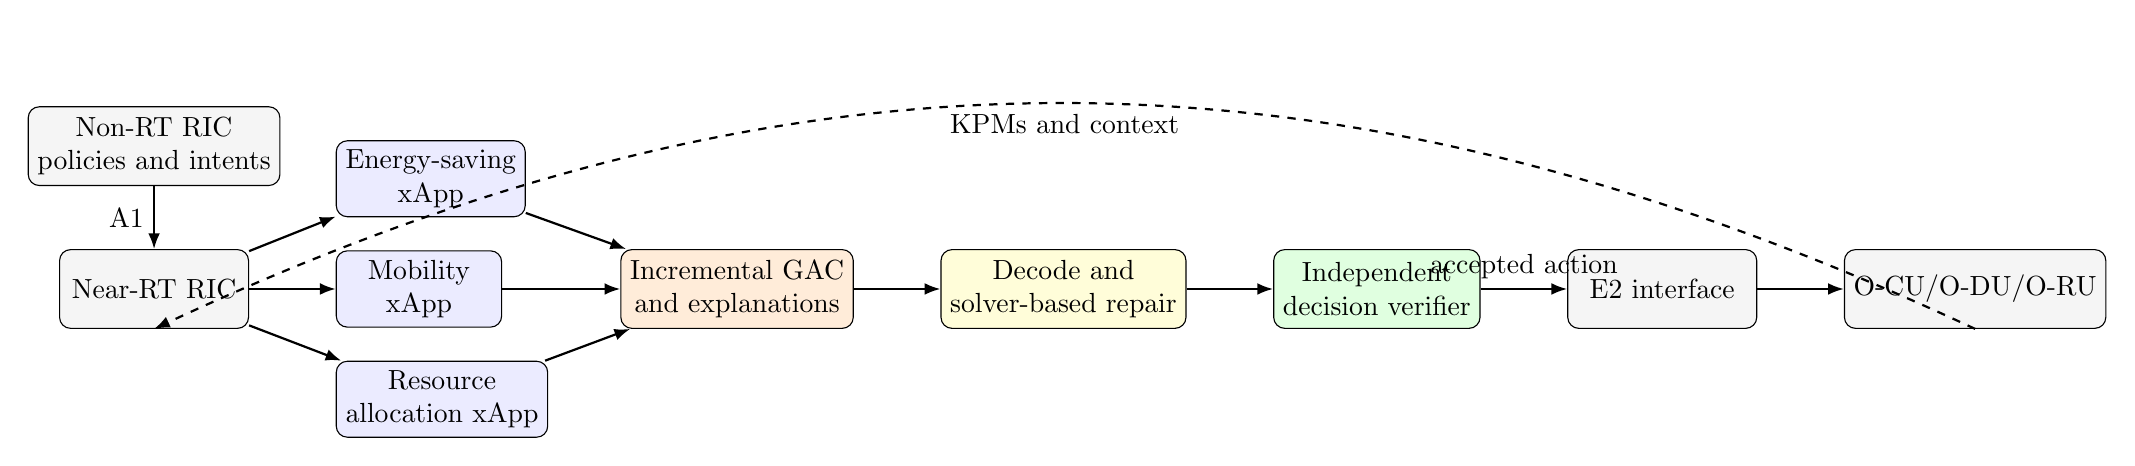
\begin{tikzpicture}[
  node distance=8mm and 11mm,
  block/.style={
    draw,
    rounded corners,
    align=center,
    minimum width=24mm,
    minimum height=10mm,
    fill=gray!8
  },
  app/.style={
    draw,
    rounded corners,
    align=center,
    minimum width=21mm,
    minimum height=9mm,
    fill=blue!8
  },
  prop/.style={
    draw,
    rounded corners,
    align=center,
    minimum width=26mm,
    minimum height=10mm,
    fill=orange!15
  },
  coord/.style={
    draw,
    rounded corners,
    align=center,
    minimum width=27mm,
    minimum height=10mm,
    fill=yellow!15
  },
  verify/.style={
    draw,
    rounded corners,
    align=center,
    minimum width=25mm,
    minimum height=10mm,
    fill=green!12
  },
  arrow/.style={
    -{Latex[length=2mm]},
    thick
  }
]

\node[block] (nonrt) {Non-RT RIC\\policies and intents};
\node[block,below=of nonrt] (near) {Near-RT RIC};

\node[app,right=of near,yshift=14mm] (x1)
  {Energy-saving\\xApp};
\node[app,right=of near] (x2)
  {Mobility\\xApp};
\node[app,right=of near,yshift=-14mm] (x3)
  {Resource\\allocation xApp};

\node[prop,right=15mm of x2] (gac)
  {Incremental GAC\\and explanations};

\node[coord,right=of gac] (coord)
  {Decode and\\solver-based repair};

\node[verify,right=of coord] (verifier)
  {Independent\\decision verifier};

\node[block,right=of verifier] (e2)
  {E2 interface};

\node[block,right=of e2] (ran)
  {O-CU/O-DU/O-RU};

\draw[arrow] (nonrt) -- node[left]{A1} (near);
\draw[arrow] (near) -- (x1);
\draw[arrow] (near) -- (x2);
\draw[arrow] (near) -- (x3);
\draw[arrow] (x1) -- (gac);
\draw[arrow] (x2) -- (gac);
\draw[arrow] (x3) -- (gac);
\draw[arrow] (gac) -- (coord);
\draw[arrow] (coord) -- (verifier);
\draw[arrow] (verifier)
  -- node[above]{accepted action} (e2);
\draw[arrow] (e2) -- (ran);

\draw[arrow,dashed]
  (ran.south)
  to[bend right=25]
  node[below]{KPMs and context}
  (near.south);

\end{tikzpicture}
}
\caption{
\method in the Near-RT RIC control path. Incremental generalized arc
consistency removes unsupported values, propagation explanations and
solver cores direct local repair, and a separately implemented
verifier gates the final action. The forwarding guarantee is relative
to the registered model and model version.
}
\label{fig:architecture}
\end{figure*}

\subsection{Incremental consistency filtering}
\label{sec:gac}

The propagator maintains a base domain $D_i$ and a filtered domain
$D_i^{*}\subseteq D_i$ for every variable. Keeping them separate is
necessary because a later relaxation may restore support for a value
that was previously removed.

For $a\in D_i$ and constraint $c$, the support set is
\begin{equation}
\begin{split}
\operatorname{Supp}_{c}
(i,a;\bm{D})
={}&
\bigl\{
\bm{z}\in R_c(\bm{s}_t):
z_i=a
\ \land\\
&\ \
z_j\in D_j,\
\forall j\in S_c
\bigr\}.
\end{split}
\label{eq:support}
\end{equation}

A hard network is generalized arc consistent when every value of
every variable has at least one support in every incident relation.
The revision operator is
\begin{equation}
\begin{split}
&\operatorname{Revise}_{c,i}(\bm{D}):
\\
&\quad
D_i
\leftarrow
\left\{
a\in D_i:
\operatorname{Supp}_{c}(i,a;\bm{D})
\neq\varnothing
\right\}.
\end{split}
\label{eq:revise}
\end{equation}

Revision is applied through a work queue until the fixed point
\begin{equation}
\bm{D}^{*}
=
\operatorname{GAC}
\left(
\bm{D},
\mathcal{C}_{\mathrm{hard}},
\bm{s}_t
\right)
\end{equation}
is reached. An empty filtered domain is a \emph{wipeout} and proves
that no feasible assignment extends the current domains. Non-empty
filtered domains do not prove global feasibility.

Across epochs, the propagator is incremental. The queue is seeded
with the constraints affected by $\Delta_t$ and constraints incident
to an affected variable. Under purely restrictive changes, cached
supports and previous deletions can be reused when their premises
remain valid. If the update contains a relaxation, the affected
constraint-graph component is restored to its base domains and
current allowed tuples before \gac is re-established. This
full-component restoration is a conservative sufficient rule; it is
not claimed to be the minimum restoration set.

For explicit positive tables, the implementation records active
tuples, the last known support of each variable--value pair, the
context identifier under which the support was valid, and the
explanation attached to each removal.

\begin{algorithm}[t]
\caption{Incremental GAC with restoration after relaxation}
\label{alg:incgac}
\small

\algin{
warm filtered domains $\bm{D}^{*}_{t-1}$,
base domains, active tables, and change set $\Delta_t$
}

\algout{
filtered domains $\bm{D}^{*}_{t}$ or \textsc{wipeout}
}

\begin{algsteps}

\item Classify $\Delta_t$ as restrictive, relaxing, mixed, or
utility-only.

\item If $\Delta_t$ contains a relaxation, restore the affected
constraint-graph component to its base domains and current allowed
tuples.

\item Apply valid restrictive deletions to the warm domains.

\item Seed the work queue with changed constraints and constraints
incident to changed variables.

\item While the queue is non-empty, remove a constraint $c$ and revise
each $i\in S_c$.

\item If some revised domain becomes empty, return \textsc{wipeout}
with its explanation.

\item Whenever a domain shrinks, enqueue the constraints incident to
that domain.

\item Return the fixed-point domains $\bm{D}^{*}_{t}$.

\end{algsteps}
\end{algorithm}

\subsection{Propagation explanations}
\label{sec:explanations}

When a value $a$ is removed from $D_i$ by constraint $c$, the
propagator records an explanation
\begin{equation}
\mathcal{E}(i,a)
\subseteq
\mathcal{C}_{\mathrm{hard}}
\cup
\mathcal{L},
\end{equation}
where $\mathcal{L}$ contains temporary domain restrictions and
boundary decisions.

The explanation contains premises sufficient to establish that every
tuple of $R_c$ assigning $a$ to $x_i$ is inactive. For each candidate
support tuple, at least one recorded premise explains why the tuple
cannot be used. A wipeout explanation is
\begin{equation}
\mathcal{E}_{\emptyset}(i)
=
\bigcup_{a\in D_i}
\mathcal{E}(i,a).
\end{equation}

Explanations are not required to be cardinality-minimal. They must be
valid relative to the registered model, reproducible from the
propagation trace, associated with a model/context identifier, and
accepted by a separate explanation checker. The checker replays the
premises and verifies that every potential supporting tuple is
disabled.

\subsection{Decoding and explanation-guided solver-based repair}
\label{sec:repair}

If propagation terminates without a wipeout, a deterministic decoder
selects
\begin{equation}
\widehat{x}_i\in D_i^{*}
\end{equation}
as the highest-utility value under a documented tie-breaking rule.
This utility decoder is intentionally conflict-unaware and is used to
isolate the contribution of repair. Section~\ref{sec:decoder-baselines}
separately evaluates conflict-aware candidate generators.

Every decoded candidate is checked against all hard relations. Let
\begin{equation}
\mathcal{C}^{0}
=
\left\{
c:
\widehat{\bm{x}}_{S_c}
\notin
R_c(\bm{s}_t)
\right\}
\end{equation}
be the initially violated relations. The initial variable core is
\begin{equation}
\mathcal{A}^{0}
=
\bigcup_{c\in\mathcal{C}^{0}}S_c.
\end{equation}

At repair iteration $r$, variables outside
$\mathcal{A}^{r}$ are fixed to their decoded values, while variables
inside the core retain their filtered domains. \gac is enforced on
the restricted model before the subproblem is submitted to \cpsat.

If propagation produces a wipeout, its explanation supplies
constraints and variables for expansion:
\begin{equation}
\mathcal{A}^{r+1}
=
\mathcal{A}^{r}
\cup
\operatorname{VarLit}
\left(
\mathcal{E}_{\emptyset}^{r}
\right)
\cup
\bigcup_{c\in\mathcal{C}^{r+1}}S_c,
\label{eq:variable-expansion}
\end{equation}
where
\begin{equation}
\mathcal{C}^{r+1}
=
\mathcal{E}_{\emptyset}^{r}
\cap
\mathcal{C}_{\mathrm{hard}}.
\end{equation}

If propagation succeeds but the restricted model is reported
\texttt{INFEASIBLE}, the assumption-core variant uses reified
boundary fixings. For each boundary variable $j$, a Boolean assumption
literal $b_j$ enforces
\begin{equation}
b_j
\Rightarrow
\left(
x_j=\widehat{x}_j
\right).
\end{equation}

The literals returned by
\texttt{SufficientAssumptionsForInfeasibility} form a sufficient, not
necessarily minimum, set of assumptions whose simultaneous activation
is inconsistent with the remaining model. The corresponding boundary
variables are released. If the returned set is empty, all currently
fixed boundary variables are conservatively released. A solver status
of \texttt{UNKNOWN} is not interpreted as infeasibility.

The core-extraction model is a feasibility model and contains no
objective. In the default explanation-guided variant, boundary values
are represented by equality constraints. If neither an explanation
nor an assumption core adds a variable, a deterministic frontier rule
adds adjacent constraints and their variables.

\begin{algorithm}[H]
\caption{Explanation-guided repair-core expansion}
\label{alg:repair}
\small

\algin{
decoded candidate $\widehat{\bm{x}}$,
registered hard model,
stage-boundary experimental budget,
and the registered fallback associated with the current model version
}

\algout{
verified local repair,
verified full-scope repair,
verified registered fallback,
or \textsc{blocked}
}

\begin{algsteps}

\item \textbf{Core feasibility phase:} Compute the violated relation set $\mathcal{C}^{0}$ and set $\mathcal{A}^{0} \leftarrow \bigcup_{c\in\mathcal{C}^{0}}S_c$.

\item For repair iteration $r=0,1,\ldots$, fix each boundary variable $j\notin\mathcal{A}^{r}$ to $\widehat{x}_j$.

\item Enforce \gac on the restricted model.

\item If propagation wipes out at the full core $\mathcal{A}^{r}=\mathcal{A}_t$, the registered hard model is infeasible; no same-model candidate, including the registered fallback, can pass the verifier, so return \textsc{blocked} for the current model version.

\item If propagation wipes out on a proper core $\mathcal{A}^{r}\subsetneq\mathcal{A}_t$, extract the wipeout explanation, expand the core, and continue.

\item Otherwise solve the objective-free restricted subproblem with \cpsat.

\item If the solver reports \texttt{INFEASIBLE} at the full core $\mathcal{A}^{r}=\mathcal{A}_t$, the registered hard model is infeasible under the current exact encoding and conclusive status; return \textsc{blocked} for the current model version.

\item If the solver reports \texttt{INFEASIBLE} on a proper core, expand the core using an assumption core when available; otherwise use the deterministic frontier rule, and continue.

\item If the solver returns \texttt{UNKNOWN}, no infeasibility conclusion is drawn; invoke the registered fallback policy and go to the verification phase with the fallback candidate.

\item If the solver returns \texttt{FEASIBLE} or \texttt{OPTIMAL}, retain the current core $\mathcal{A}^{r}$ and break to the optimization phase.

\item \textbf{Operational optimization phase:} Optimize the lexicographic objectives on the feasible core. If every active lexicographic level returns \texttt{OPTIMAL}, mark the repair \textsc{lex-optimal}. If the budget expires with a verified feasible incumbent before all levels are certified, mark it \textsc{feasible-not-certified} and submit the incumbent to the verification phase.

\item \textbf{Verification phase:} Submit the final optimized or fallback candidate to the independent verifier. If the verifier accepts it, return the verified candidate. If it rejects an optimized candidate, submit the registered fallback to the verifier; if the fallback is accepted, return it. Otherwise return \textsc{blocked}.

\end{algsteps}
\end{algorithm}

Each repair emits a repair certificate containing the model and
context identifiers, decoded candidate, initial violation witnesses,
repair-core sequence, source of every expansion, released boundary
variables, final assignment, solver status, and verifier outcome.
Propagation explanations and solver assumption cores are included
when they cause an expansion.

Certificate replay checks that the initial candidate violates the
listed relations, each expansion follows the recorded rule, and the
final assignment satisfies every registered hard constraint.
Therefore, the certificate is an audit trace. It does not by itself
prove minimum core size or global objective optimality. The present
evaluation did not separately measure serialized certificate size or
replay latency.

The intended repair preference order is lexicographic:

\begin{enumerate}
\item satisfy every hard relation;
\item minimize weighted reconfiguration against the previous verified
decision;
\item minimize deviation from the decoded candidate;
\item maximize static utility.
\end{enumerate}

Hard feasibility is not scalarized with the soft levels. A
\texttt{FEASIBLE} solver status establishes feasibility but does not
establish objective optimality. A claim of global objective
optimality requires a corresponding \texttt{OPTIMAL} status for the
encoded complete model. Accordingly, this paper uses
the term \emph{solver-based repair} for the \cpsat-based repair
engine. The evaluation therefore reserves \emph{certified optimum}
for solutions proven optimal across all active lexicographic levels.

A fallback must be explicitly registered in the current model, for
example rejection of the conflicting requests, retention of a
previous configuration, or a safe no-operation. It must pass the same
verifier as any solver-generated candidate. The previous
configuration is therefore re-verified before reuse. If the complete
registered hard model is infeasible, no fallback belonging to that
model can be accepted; the pipeline therefore returns
\textsc{blocked} for that model version.

\subsection{Independent verification}
\label{sec:verifier}

The production verifier is implemented separately from propagation,
explanation construction, and repair. It receives the model/context
identifier, selected actions, base domains, hard relations, and SLA
thresholds. It accepts the registered feasible set
\begin{equation}
\begin{split}
\mathcal{F}(\bm{s}_t)
={}&
\bigl\{
\bm{x}:
x_i\in D_i
\ \land\\
&\ \
\bm{x}_{S_c}\in R_c(\bm{s}_t),
\
\forall c\in\mathcal{C}_{\mathrm{hard}}
\bigr\}.
\end{split}
\label{eq:feasible-set}
\end{equation}

\begin{proposition}[Registered-model forwarding soundness]
\label{prop:soundness}
Assume that the production verifier accepts exactly the assignments in
$\mathcal{F}(\bm{s}_t)$, forwarding is enabled only after verifier
acceptance, and the registered model version does not change between
verification and forwarding. Then every forwarded action belongs to
$\mathcal{F}(\bm{s}_t)$ for that registered model version.
\end{proposition}

\begin{proof}
The verifier checks the membership of every selected value in its base
domain and checks every registered hard relation. The forwarding gate
rejects any candidate that fails one of these checks. Model-version
binding prevents acceptance under one registered model from being
reused after the model changes.
\end{proof}

Proposition~\ref{prop:soundness} is an architectural invariant
conditional on verifier correctness, complete registration of the
hard constraints, and atomic model-version handling. It does not
imply that the registered model captures every dependency of the
physical RAN.

\subsection{Verifier-validation gates}

The verifier is evaluated through four validation gates.

\begin{itemize}

\item \textbf{G1: exhaustive oracle comparison.}
Every assignment of randomly generated small instances is enumerated
and classified by an independently coded oracle.

\item \textbf{G2: triple agreement.}
A declarative \cpsat model is reconstructed from a JSON-normalized
representation using a separate parser. The production verifier,
oracle, and declarative implementation must agree.

\item \textbf{G3: property-based testing.}
The tests cover determinism, constraint-order invariance,
variable-renaming invariance, and rejection of out-of-domain values,
missing variables, and stale contexts.

\item \textbf{G4: oracle-labelled input mutation.}
Mutants of planted-feasible assignments are classified independently
by the oracle. A mutant that remains feasible is labelled feasible;
the test does not assume that every mutation must create an invalid
assignment.

\end{itemize}

The oracle and second verifier share no relation parser, tuple
normalizer, domain-indexing routine, or context-validation routine
with the production verifier. A separate serializer produces the
normalized representation consumed by G2. A divergence at any gate
blocks the corresponding campaign. Zero divergence increases
confidence in the tested implementation but does not prove correctness
for all possible inputs.

\subsection{Safety, availability, and timeliness}
\label{sec:timing-semantics}

Three properties must be distinguished.

\emph{Safety} means that no candidate rejected by the
registered-model verifier is forwarded. \emph{Availability} means
that the pipeline produces a verifier-accepted action, including an
accepted fallback. \emph{Timeliness} means that such an action becomes
available before the control deadline.

The forwarding architecture enforces safety relative to the registered
model. Availability is not unconditional because the registered hard
model or every fallback may be infeasible. The temporal metrics distinguish four boundaries: (1) \cpsat's internal 100~ms solver time limit; (2) stage-boundary budget checks, where an algorithm inspects elapsed time before invoking a subsequent stage; (3) post-hoc deadline-compliance classification, which labels an outcome based on total elapsed time; and (4) the absence of preemptive interruption, meaning a running stage (such as propagation) is allowed to complete before its latency is recorded. Consequently, the experiments characterize
computational latency and post-hoc compliance; they do not demonstrate
a hard real-time scheduling guarantee.

% ============================================================
\section{Analysis}
\label{sec:analysis}
% ============================================================

\begin{proposition}[Solution preservation]
\label{prop:preservation}
\[
\forall \bm{x}\in\mathcal{F}(\bm{s}_t),\ \forall i\in\mathcal{A}_t,\quad x_i\in D_i^{*}.
\]
Thus, \gac filtering removes no value used by a globally feasible assignment.
\end{proposition}

\begin{proof}
A value is removed only if it has no support under the current
domains. Suppose $\bm{x}$ is feasible and $x_i=a$. For every hard
constraint $c$ incident to $i$, the tuple
$\bm{x}_{S_c}\in R_c(\bm{s}_t)$ supports $a$ as long as all its
components remain in their current domains. Initially, every
component is present. By induction over the revision sequence, no
component of $\bm{x}$ can be the first removed component because the
remaining components of the same feasible tuple would still support
it.
\end{proof}

Filtering alone does not guarantee valid decoding. Consider

\[
D_1=D_2=\{0,1\}
\]
with

\[
R_{\neq}=\{(0,1),(1,0)\}.
\]
Every value has support, so the network is \gac. A deterministic
per-variable decoder that resolves both symmetric ties identically
returns either $(0,0)$ or $(1,1)$, both of which violate
$R_{\neq}$. Propagation and repair therefore address different
failure modes.

\begin{proposition}[Monotone expansion and conditional completeness]
\label{prop:completeness}
The repair cores satisfy

\[
\mathcal{A}^{0}
\subseteq
\mathcal{A}^{1}
\subseteq
\cdots
\subseteq
\mathcal{A}_t.
\]
If every unsuccessful non-full iteration adds at least one variable,
the full set is reached after at most
$|\mathcal{A}_t|-|\mathcal{A}^{0}|$ expansions. If the full core is
reached, all finite-domain relations are encoded correctly, the solver
returns a conclusive status before its time limit, and the solver is
complete for that model, then the repair stage returns a feasible
assignment if and only if the registered hard model is feasible.
\end{proposition}

\begin{proof}
Monotonicity follows from the expansion rule, which only adds
variables. The expansion bound follows because every unsuccessful
non-full iteration adds at least one previously absent variable. At
the full core, no boundary variable is fixed, so the repair model
coincides with the complete hard model. The result then follows from
the assumed completeness and conclusive solver status.
\end{proof}

A repair restricted to a proper subset is not complete. Its
infeasibility may result from the fixed boundary even if the complete
model is feasible. Therefore, local infeasibility is never reported as
global model infeasibility.

\begin{proposition}[Restoration after relaxation]
\label{prop:restoration}
Suppose value $a$ was removed at epoch $t-1$ because it had no support
in $R_c(\bm{s}_{t-1})$. If the relation is relaxed at epoch $t$,
retaining the deletion without re-evaluation may exclude a feasible
assignment of $\mathcal{M}_t$.
\end{proposition}

\begin{proof}
The relaxed relation may introduce a tuple
$\bm{z}\in R_c(\bm{s}_t)$ such that $z_i=a$ and all other tuple
components belong to their current domains. Then $\bm{z}$ is a new
support for $a$, so the previous no-support explanation is no longer
valid.
\end{proof}

A complete scan of explicit positive tables admits the coarse per-scan bound
\begin{equation}
O\left(
\sum_{c}
|R_c|\,|S_c|
\right).
\end{equation}
Actual propagation time depends on support caching, tuple activity,
arity, and the number of removals. Memory use includes the positive
tables, active-tuple state, support caches, explanations, and
certificates. Solver-based repair remains exponential in the worst
case. Core expansion may reach the complete variable set, at which
point the localization advantage disappears.

% ============================================================
\section{Experimental Setup}
\label{sec:experiments}
% ============================================================

\subsection{Simulator, scenarios, and instance suites}

The evaluation uses a Python-based O-RAN coordination simulator
containing instance generators, an observable \gac propagator,
explanation recorder and checker, OR-Tools \cpsat adapters, the repair
engine, the independent verifier, and a pseudo-physical network model.

The pseudo-physical model maps power, resource-block fraction,
handover offset, and sleep-state decisions to SINR, throughput, energy
per bit, Jain fairness, and a handover-failure indicator. Users are
placed uniformly and path loss is distance based. The model is
intended to provide reproducible KPMs, not to replace a system-level
or closed-loop O-RAN simulator.

Generated relations encode KPM thresholds, ownership rules, and
sleep/wake exclusivity. Each generated feasible test instance retains
a planted feasible assignment so that coordination failure can be
distinguished from instance infeasibility. A separate diagnostic suite
contains controlled infeasible instances for wipeout and explanation
tests.

Table~\ref{tab:scenarios} summarizes the five scenarios. They contain
12--30 action variables with domain sizes of three or four and 50
seeds per scenario, giving 250 matched static instances.

\begin{table*}[t]
\centering
\caption{Generated O-RAN coordination scenarios.}
\label{tab:scenarios}
\setlength{\tabcolsep}{4pt}
\small

\begin{tabular}{
  >{\raggedright\arraybackslash}p{18mm}
  >{\raggedright\arraybackslash}p{27mm}
  >{\raggedright\arraybackslash}p{32mm}
  >{\raggedright\arraybackslash}p{32mm}
  >{\raggedright\arraybackslash}p{36mm}
}
\toprule
Scenario &
xApps &
Controlled parameters &
Principal KPMs &
Conflict mechanism\\
\midrule

S1: direct power conflict &
Coverage and energy-saving &
Transmission power, cell state &
Coverage, SINR, energy &
Incompatible requests on the same parameter\\

S2: radio-resource conflict &
Power-control and resource-allocation &
Power level, resource-block profile &
Throughput, interference, loss &
Different parameters influencing common KPMs\\

S3: mobility--energy conflict &
Mobility-robustness and energy-saving &
Handover offsets, sleep/wake &
Handover failures, ping-pong, energy &
Sleep decisions modify coverage and mobility\\

S4: load-balancing conflict &
Load-balancing and mobility &
Cell offsets, handover thresholds &
Cell load, edge throughput, handovers &
Joint control of user association\\

S5: multi-xApp stress &
All xApps &
Joint action space &
All registered KPMs and SLAs &
Mixed direct, indirect, and implicit relations\\

\bottomrule
\end{tabular}
\normalsize
\end{table*}

The dynamic suite runs the five scenarios over 30 episodes of 100
epochs, giving 15{,}000 epochs. A fixed schedule contains restrictive,
relaxing, mixed, and utility-only transitions that modify 1--50\% of
the model. Mixed transitions account for 84\% of the schedule.
Restrictive, relaxing, and utility-only transitions are included as
isolated diagnostic cases.

The repair-stress suite contains 50 planted-feasible instances with
24 variables, domain size four, 34 relations, and 70\%
equality-type constraints. The candidate is generated by flipping
three variables of the planted solution.

The cold-start suite contains instances with

\[
n\in\{30,100,300,600,1000\},
\quad
d=6,
\quad
|\mathcal{C}|=2n,
\]
table tightness 0.25, and 20 seeds per size.

The sequential suite contains ten episodes of 30 epochs per size and
change rate. Between epochs, a fraction

\[
\delta\in\{2\%,10\%\}
\]
of the relations is re-randomized while retaining a planted feasible
assignment. A drift variant re-plants 1\% of the variables per epoch.

These generators produce controlled finite-domain workloads. They do
not establish representativeness for dense, high-arity, adversarial,
or commercial multi-vendor RAN models.

\subsection{Operational repair objective and solver configuration}

The core-extraction model focuses exclusively on feasibility to isolate conflicts, containing no objective function. The subsequent operational repair stage implements the lexicographic preference defined in Section~\ref{sec:repair} via sequential solves. We determine the optimum for each objective level sequentially:
\begin{equation}
z_1^\star = \min_{x \in \mathcal{F}(\bm{s}_t)} H(x, x^{t-1})
\end{equation}
\begin{equation}
z_2^\star = \min_{\substack{x \in \mathcal{F}(\bm{s}_t) \\ H(x, x^{t-1}) = z_1^\star}} D(x, \hat{x})
\end{equation}
\begin{equation}
z_3^\star = \max_{\substack{x \in \mathcal{F}(\bm{s}_t) \\ H = z_1^\star \\ D = z_2^\star}} U_{\mathrm{int}}(x, s_t)
\end{equation}
where $H$ is the weighted reconfiguration distance, $D$ is the deviation from the decoded candidate $\hat{x}$, and $U_{\mathrm{int}}$ is the scaled static utility. 

To comply with \cpsat's exact-integer requirements, continuous utility values and fractional weights are scaled by $10^4$ and rounded to integers. The total 100~ms solver time allocation is shared sequentially: each CP-SAT call receives the remaining solver budget $B_{k+1}=\max\{0,B_k-\tau_k\}$, rather than the original full budget. The implementation applies the objective levels sequentially. A subsequent level is optimized only after the preceding level has returned \texttt{OPTIMAL}; the certified optimum value is then imposed as an equality constraint. If a stage returns \texttt{FEASIBLE} because its budget expires, the incumbent may be accepted after independent verification, but neither that objective level nor the complete lexicographic sequence is considered optimal. Such outcomes are reported as feasible repairs without an objective-optimality certificate. For tie-breaking, the utility decoder selects the highest utility, then lowest action index. For solver-generated repairs, tied optima are considered equivalent and any tied solution may be returned.

\begin{table*}[t]
\centering
\caption{Solver configurations per campaign environment. For static and dynamic scenarios, standard Windows multiprocessing scaling was used with non-fixed (default) random seeds.}
\label{tab:solver-config}
\setlength{\tabcolsep}{4pt}
\small
\begin{tabular}{lrrlll}
\toprule
Campaign & OR-Tools & Workers & Seed & Limit & Presolve \\
\midrule
Static & 9.14 & 28 & default/not fixed & none & enabled \\
Dynamic & 9.14 & 28 & default/not fixed & none & enabled \\
Repair ablation & 9.15 & 1 & 1 & 100 ms shared & enabled \\
Sequential & 9.15 & 1 & 1 & 100 ms shared & enabled \\
\bottomrule
\end{tabular}
\end{table*}

Table~\ref{tab:solver-config} lists the execution environments. The repair-ablation and sequential campaigns in the secondary Linux environment enforced reproducible single-threaded execution (\texttt{num\_search\_workers = 1}) with deterministic seeds, eliminating portfolio-search variance. In contrast, the static campaign did not strictly control garbage collection, CPU affinity, or execution order across the 28 workers, and effective seeds varied by process; its latency results therefore include this system-level variability. Warm-up runs were executed prior to measurement to initialize the runtime environment. Building the model and extracting the solution are included in the reported solver latencies, whereas independent verification is measured separately.

\subsection{Structural characterization}

The synthetic instances exhibit structural properties conducive to local repair. The constraint graph has a mean degree of 3.4 and maximum degree of 8, with relations having arities of 2 or 3. This sparse clustering may favour localized propagation and repair and therefore limits the generalizability of the sequential results.

\subsection{Compared methods}

All methods share the same registered input model, timing harness, and
final verifier.

The comparison includes:

\begin{itemize}

\item uncoordinated forwarding;

\item static priority;

\item \gac followed by utility decoding without repair;

\item complete \cpsat rebuilt from the full model;

\item \gac followed by full \cpsat;

\item \method using \gac, utility decoding, expanding repair, and
verification;

\item continuous-relaxation variants;

\item fixed violated-scope repair;

\item radius-based repair;

\item frontier core repair;

\item explanation-guided repair;

\item assumption-core repair;

\item full-scope repair;

\item a QoS-inspired kept-request optimizer;

\item a discretized Nash-social-welfare optimizer;

\item greedy, min-conflicts, and forward-checking candidate generators.

\end{itemize}

The QoS-aware and bargaining baselines reproduce objective structures
inspired by previous work
\cite{wadud2024qacm,wadud2023game}; they are not reimplementations of
the complete published systems.

In the sequential suite, the incremental candidate is the previous
verified decision. It is re-verified under the updated model and
repaired if necessary. The competing solver baselines rebuild and
re-solve the full \cpsat model, either without a hint or with the
previous solution supplied as a hint. Thus, the comparison is against
the evaluated Python rebuild-and-resolve implementations, not against
every possible persistent or incremental solver architecture.

\subsection{Outcome terminology}

\begin{table*}[t]
\centering
\caption{Decision-outcome terminology.}
\label{tab:terminology}
\setlength{\tabcolsep}{4pt}
\small
\begin{tabular}{ll}
\toprule
Term & Meaning\\
\midrule
Direct decode & Candidate accepted without repair\\
Local repair & Candidate corrected using a proper subset of variables\\
Full-scope repair & Repair after expansion to the complete model\\
Fallback & Registered fallback accepted by the verifier\\
Blocked & No verifier-accepted action produced\\
Verified feasibility & Direct, local, full-scope, or verified fallback outcome\\
Deadline compliance & Verified action completed within the post-hoc threshold\\
\bottomrule
\end{tabular}
\end{table*}

Verified feasibility includes only actions accepted by the final
verifier. A fallback is reported separately and is not silently
counted as an optimized solution.

The 100~ms threshold is a post-hoc compliance metric checked after
propagation, decoding, repair iterations, and verification. It is not
a preemptive interrupt. Therefore, the experiments do not demonstrate
hard real-time schedulability.

\subsection{Metrics and statistical protocol}

Filtering is measured using
\begin{equation}
r_D
=
1-
\frac{\sum_i|D_i^{*}|}
     {\sum_i|D_i|}
\end{equation}
and
\begin{equation}
r_R
=
1-
\frac{\sum_c|R_c^{*}|}
     {\sum_c|R_c|},
\end{equation}
where $R_c^{*}$ is the active part of relation $R_c$ after
propagation.

Binary paired outcomes are reported as counts and compared using
exact McNemar tests. Continuous paired outcomes are summarized using
medians, paired Wilcoxon signed-rank tests, and matched-pairs
rank-biserial correlations. All statistical analyses were executed in the Python 3.10 Linux environment using \texttt{scipy.stats} (SciPy 1.11.0) and \texttt{statsmodels.stats.multitest} (Statsmodels 0.14.0), irrespective of the environment used to generate each campaign's raw measurements. Holm
correction is applied within the declared comparison families (Table~\ref{tab:families}).
Statistical operations were implemented as follows:
\begin{itemize}
\item Wilcoxon signed-rank tests: \texttt{scipy.stats.wilcoxon} (SciPy 1.11.0).
\item McNemar tests: \texttt{scipy.stats.binomtest} applied to discordant pairs (SciPy 1.11.0).
\item BCa intervals: \texttt{scipy.stats.bootstrap} (SciPy 1.11.0).
\item Holm adjustment: \texttt{multipletests} from \texttt{statsmodels.stats.multitest} (Statsmodels 0.14.0).
\item Rank-biserial correlation: custom exact formula implementation (provided in the artifact).
\item Hodges--Lehmann estimate: custom Walsh-average implementation (provided in the artifact).
\end{itemize}
Bootstrap 95\% confidence intervals for paired medians are computed using the paired-difference BCa resampling procedure with 10{,}000 replicates and seed 1. Marginal KPM confidence intervals are computed using a separate decision-level BCa bootstrap, also with 10{,}000 replicates.

\begin{table*}[t]
\centering
\caption{Multiple-hypothesis correction families. Statistical significance claims are adjusted within these predefined families using the Holm--Bonferroni method. The $p$-values are reported for the primary confirmatory tests. For McNemar comparisons, $b$ and $c$ denote the off-diagonal discordant pairs: $b=\#(A\text{ succeeds},B\text{ fails})$ and $c=\#(A\text{ fails},B\text{ succeeds})$.}
\label{tab:families}
\setlength{\tabcolsep}{3.5pt}
\small
\begin{tabular}{llllrrrrr}
\toprule
Family & Outcome & Method A & Method B & $N$ & $b$ & $c$ & Raw $p$ & Adjusted $p$ \\
\midrule
F1a & End-to-end verified feasibility & \cpsat & \method & 250 & 0 & 0 & 1.000 & 1.000 \\
    & End-to-end verified feasibility & Continuous & \method & 250 & 0 & 7 & 0.016 & 0.031 \\
\midrule
F1b & Direct decoder feasibility & Min-conflicts & Utility decoder & 250 & 177 & 0 & $1.0\cdot 10^{-53}$ & $2.1\cdot 10^{-53}$ \\
    & Direct decoder feasibility & Forward check & Utility decoder & 250 & 213 & 0 & $1.5\cdot 10^{-64}$ & $4.6\cdot 10^{-64}$ \\
    & Direct decoder feasibility & Greedy & Utility decoder & 250 & 14 & 2 & $4.2\cdot 10^{-3}$ & $4.2\cdot 10^{-3}$ \\
\midrule
F2 & Repair success & Radius-zero & Explanation & 248 & 0 & 21 & $9.5\cdot 10^{-7}$ & $2.9\cdot 10^{-6}$ \\
   & Repair success & Violated-scope & Explanation & 248 & 0 & 21 & $9.5\cdot 10^{-7}$ & $2.9\cdot 10^{-6}$ \\
   & Repair success & Frontier & Explanation & 248 & 0 & 0 & 1.000 & 1.000 \\
\midrule
F3 & Repair latency & Full solve & Explanation & 248 & -- & -- & $8.0\cdot 10^{-34}$ & $8.0\cdot 10^{-34}$ \\
\midrule
F4 & Core size & Radius-zero & Explanation & 248 & -- & -- & $4.7\cdot 10^{-5}$ & $1.4\cdot 10^{-4}$ \\
   & Core size & Violated-scope & Explanation & 248 & -- & -- & $4.7\cdot 10^{-5}$ & $1.4\cdot 10^{-4}$ \\
   & Core size & Frontier & Explanation & 248 & -- & -- & $3.4\cdot 10^{-3}$ & $3.4\cdot 10^{-3}$ \\
\midrule
F5 & Seq. latency 2\%/100 & Re-solve & \method & 10 & -- & -- & 0.001953 & 0.007812 \\
   & Seq. latency 2\%/300 & Re-solve & \method & 10 & -- & -- & 0.001953 & 0.007812 \\
   & Seq. latency 2\%/600 & Re-solve & \method & 10 & -- & -- & 0.001953 & 0.007812 \\
   & Seq. latency 2\%/1000 & Re-solve & \method & 10 & -- & -- & 0.001953 & 0.007812 \\
\bottomrule
\end{tabular}
\end{table*}

In the sequential suite, the episode is the inferential unit for
median-latency comparisons because epochs from the same episode are
temporally dependent. Epoch-level p95, p99, and maximum values are
reported descriptively. With ten episodes of 30 epochs, especially
the p99 estimate is based on very few extreme observations and should
not be interpreted as a precise tail model.

Timeouts are treated as censored outcomes and are not converted into
ordinary latency observations.

\subsection{Execution environments}

The scenario, dynamic, and temporal campaigns ran on the primary
reference host: a 28-core Intel system under Windows~11, Python~3.13,
and OR-Tools~9.14.

The operational-candidate ablation, cold-start, sequential,
objective-gap, baseline, and verifier-validation campaigns ran in a
2-vCPU Linux container using Python~3.10 and OR-Tools~9.15.

All paired comparisons are within an environment. Absolute latency
values from different environments are not directly compared. The
artifact records the versions, seed hierarchy, and commands. A
single-host rerun remains desirable before deployment conclusions are
drawn.

% ============================================================
\section{Results}
\label{sec:results}
% ============================================================

\subsection{Trust layer}

All four verifier-validation gates passed with zero divergence
(Table~\ref{tab:gates}). The total comprised 60{,}650 exhaustive
assignment comparisons, 1{,}800 triple-agreement checks, 602{,}000
property-based checks, and 16{,}000 oracle-labelled input mutants.

\begin{table*}[t]
\centering
\caption{Verifier-validation gates.}
\label{tab:gates}
\setlength{\tabcolsep}{4pt}
\small

\begin{tabular}{llrr}
\toprule
Gate & Content & Checks & Divergences\\
\midrule
G1 & Exhaustive oracle comparison & 60{,}650 & 0\\
G2 & Triple agreement with \cpsat & 1{,}800 & 0\\
G3 & Property-based testing & 602{,}000 & 0\\
G4 & Oracle-labelled mutants & 16{,}000 & 0\\
\midrule
& Total & 680{,}450 & 0\\
\bottomrule
\end{tabular}
\end{table*}

On small instances for which exhaustive enumeration was practical, no
value removed by propagation belonged to a feasible assignment.
Incremental propagation reproduced the domains obtained by full
recomputation on all 15{,}000 dynamic epochs. The explanation checker
accepted 15{,}000 valid generated explanations (covering both wipeout and ordinary value-removal explanations) and rejected 15{,}000 synthetically corrupted counterparts (using random value-removal operators) with zero false accepts and zero false rejects. Operational repair certificates are implemented and replayable but their quantitative serialization overhead was not formally evaluated.

These tests support the implementation-level trust argument but do
not validate the registered model against a physical RAN and do not
prove verifier correctness outside the tested input distributions.

\subsection{Consistency filtering}

Propagation removed 21.7\% of candidate values and 34.1\% of relation
tuples when pooled over the static suite. Median \gac latency remained
below 0.3~ms in every scenario.

\begin{table*}[t]
\centering
\caption{
Consistency-propagation results over 50 generated instances per
scenario.
}
\label{tab:propagation-results}
\setlength{\tabcolsep}{3.5pt}
\small

\begin{tabular}{lrrrrrrrr}
\toprule
Scenario &
Values before &
Values after &
$r_D$ (\%) &
Tuples before &
Tuples after &
$r_R$ (\%) &
Median (ms) &
P95 (ms)\\
\midrule

S1 & 1800 & 1414 & 21.4 & 2403 & 1713 & 28.7 & 0.07 & 0.09\\
S2 & 3600 & 2676 & 25.7 & 6083 & 3697 & 39.2 & 0.15 & 0.18\\
S3 & 4000 & 3148 & 21.3 & 7419 & 4858 & 34.5 & 0.17 & 0.20\\
S4 & 4800 & 3908 & 18.6 & 9694 & 6846 & 29.4 & 0.20 & 0.24\\
S5 & 6000 & 4662 & 22.3 & 11747 & 7488 & 36.3 & 0.26 & 0.31\\

\bottomrule
\end{tabular}
\normalsize
\end{table*}

\begin{figure}[t]
\centering

\includegraphics[
  width=\columnwidth
]{artifacts/figures/fig1_reduction.pdf}
\caption{
Domain and relation-table reductions obtained by generalized arc
consistency.
}
\label{fig:domain-reduction}
\end{figure}

\subsection{Static-suite feasibility and latency}

Table~\ref{tab:main-results} reports integer decision outcomes. The
conflict-unaware utility decoder directly produced a valid joint
assignment on only 2 of 250 instances. \method repaired the remaining
248 candidates and achieved 100\% verified feasibility.

Complete \cpsat and \gac followed by full \cpsat also achieved 100\%
verified feasibility. Their median latencies were 2.8 and 2.6~ms,
respectively, compared with 1.8~ms for \method.

\begin{table*}[t]
\centering
\caption{
End-to-end outcomes on the static suite. Deadline compliance is
post-hoc. The \emph{Uncoordinated} and \emph{Static priority} rows
carry no verifier and are blocked on all 250 instances by
construction; they are reported as sanity checks rather than as
competing coordination methods.
}
\label{tab:main-results}
\setlength{\tabcolsep}{3pt}
\footnotesize

\begin{tabular}{lrrrrrrrrrr}
\toprule
Method &
$N$ &
Direct &
Local &
Full &
Fallback &
Blocked &
Feasible &
$\leq100$ ms &
Median &
P95\\
&
&
&
repair &
scope &
&
&
(\%) &
(\%) &
(ms) &
(ms)\\
\midrule

Uncoordinated
& 250 & 0 & 0 & 0 & 0 & 250 & 0.0 & 0.0 & 0.0 & 0.1\\

Static priority
& 250 & 0 & 0 & 0 & 0 & 250 & 0.0 & 0.0 & 0.0 & 0.0\\

\gac + utility decode
& 250 & 2 & 0 & 0 & 0 & 248 & 0.8 & -- & -- & --\\

\cpsat
& 250 & 0 & 0 & 250 & 0 & 0 & 100.0 & 100.0 & 2.8 & 4.8\\

\gac + \cpsat
& 250 & 2 & 0 & 248 & 0 & 0 & 100.0 & 100.0 & 2.6 & 4.7\\

\textbf{\method}
& 250 & 2 & 248 & 0 & 0 & 0 &
\textbf{100.0} &
\textbf{100.0} &
\textbf{1.8} &
\textbf{3.8}\\

\midrule

Continuous only
& 250 & 189 & 0 & 0 & 0 & 61 & 75.6 & 23.6 & 180.4 & 365.7\\

\gac + continuous decode
& 250 & 186 & 0 & 0 & 0 & 64 & 74.4 & 44.4 & 80.6 & 251.3\\

Continuous + repair (explanation)
& 250 & 186 & 57 & 0 & 0 & 7 & 97.2 & 57.4 & 79.9 & 253.3\\

Continuous + repair (radius)
& 250 & 186 & 57 & 0 & 0 & 7 & 97.2 & 57.0 & 82.6 & 251.9\\

Continuous + repair (assumption)
& 250 & 186 & 58 & 0 & 0 & 6 & 97.6 & 57.8 & 81.3 & 254.4\\

\bottomrule
\end{tabular}
\normalsize
\end{table*}

The paired median difference between \method and complete \cpsat was
$-0.85$~ms, with a bootstrap 95\% interval
$[-0.93,-0.72]$~ms. The paired Wilcoxon result was
$p\approx 7\cdot 10^{-34}$ and the matched-pairs rank-biserial correlation was $-0.89$.
This difference is statistically significant under the specified paired test, although operationally modest in magnitude.

\begin{table*}[t]
\centering
\caption{
Final certification status of completed lexicographic repair
sequences. A decision or epoch is LEX-OPTIMAL when every
lexicographic level of its repair returned \texttt{OPTIMAL};
FEASIBLE-NOT-CERTIFIED denotes a verifier-accepted incumbent
returned before full lexicographic certification. An episode is
counted as LEX-OPTIMAL only if every repaired epoch in that episode
achieved complete lexicographic certification. Counts are completed
repair sequences, not internal solver calls; each sequence comprises
one or more core-feasibility calls followed by up to three
objective-level optimizations.
}
\label{tab:epoch-status}
\setlength{\tabcolsep}{4pt}
\small
\begin{tabular}{llrrr}
\toprule
Campaign & Unit & \shortstack[l]{Completed\\repairs} & \shortstack[l]{LEX-\\OPTIMAL} & \shortstack[l]{FEASIBLE-NOT-\\CERTIFIED} \\
\midrule
Static repair & decisions & 248 & 248 & 0 \\
Dynamic repair & epochs & 14{,}755 & 14{,}755 & 0 \\
Sequential F5 confirmatory subset & episodes & 40 & 40 & 0 \\
\bottomrule
\end{tabular}
\end{table*}

\begin{table*}[t]
\centering
\caption{
Paired static-instance comparisons. Latency effect sizes are
matched-pairs rank-biserial correlations. HL denotes the
Hodges--Lehmann paired difference in milliseconds.
}
\label{tab:stats-paired}
\setlength{\tabcolsep}{3pt}
\small

\begin{tabular}{lrrrrrrrrr}
\toprule
Comparison &
$N$ &
Feasibility A/B &
$b$ & $c$ &
$p_{\mathrm{McN}}$ &
Median A/B &
HL &
$p_{\mathrm{Wilc}}$ &
$r_{\mathrm{rb}}$\\
\midrule

\method vs \cpsat
& 250 & 100/100 & 0 & 0 & -- & 1.76/2.76 &
$-0.85$ & $<10^{-33}$ & $-0.89$\\

\method vs \gac+\cpsat
& 250 & 100/100 & 0 & 0 & -- & 1.76/2.63 &
$-0.75$ & $<10^{-30}$ & $-0.85$\\

Continuous+repair vs \method
& 250 & 97.2/100 & 0 & 7 & 0.031 & 79.9/1.75 &
$+94$ & $<10^{-40}$ & $+1.0$\\

Continuous+repair vs \cpsat
& 250 & 97.2/100 & 0 & 7 & 0.031 & 79.9/2.76 &
$+93$ & $<10^{-40}$ & $+1.0$\\

\bottomrule
\end{tabular}
\normalsize
\end{table*}

The objective-inspired baselines also achieved 100\% verified
feasibility and retained approximately 64\% of preferred actions.
Their latency results were obtained in the secondary environment and
are not directly compared with results from the primary host.

The continuous-relaxation stage was counterproductive on this suite.
It increased median latency to approximately 80~ms, reduced post-hoc
deadline compliance to approximately 57\%, and left six or seven
instances blocked, depending on the core rule. Its feasibility deficit relative to the discrete pipeline was statistically significant (exact McNemar $p=0.016$ unadjusted, $p_{\mathrm{Holm}}=0.031$). It was therefore
excluded from the proposed operational pipeline.

For the continuous-relaxation evaluations, the upstream end-to-end coordination feasibility sample size is strictly $N=250$. However, the downstream KPM-analysis sample is $N=249$ because one verifier-accepted decision failed during the post-verification KPM simulation stage due to a simulator numerical error. A post-verification simulator error does not constitute a failure of the upstream coordination pipeline. The failed simulation concerns a single S5 instance that was verifier-accepted under both \method and the continuous variants; the \cpsat KPM simulation on the same generated instance completed, so its marginal sample remains $n=250$, whereas the \method sample excludes that instance ($n=249$) and the explanation-guided continuous sample excludes it as well ($n=242$ of its 243 verifier-accepted decisions). Missing simulator values were omitted pairwise in computations using decisions as the resampling unit, and all KPM intervals are marginal decision-level bootstrap intervals rather than paired-sample intervals.

\subsection{Repair-core ablation}

Table~\ref{tab:repair-results} compares repair-core strategies on all 248 repair candidates produced by the conflict-unaware utility decoder on the static suite. Fixed violated-scope and radius-zero repair succeeded on 227 of 248 cases (91.5\%), whereas the expanding variants succeeded on all 248. The exact paired McNemar comparison between explanation-guided and radius-zero repair contained 21 discordant pairs, all favouring explanation-guided repair ($b=0$, $c=21$), giving $p_{\mathrm{raw}}=9.5\cdot 10^{-7}$ and $p_{\mathrm{Holm}}=2.9\cdot 10^{-6}$ within family F2. The success-rate advantage of core expansion over fixed-scope repair is therefore statistically significant on this suite. This advantage is attributable to expansion itself rather than to explanation guidance specifically: the frontier, assumption-core, and full-scope strategies also resolved all 248 candidates. The specific benefit of explanation guidance is that it recovered the 21 missed candidates with markedly smaller final cores than full-scope solving.

\begin{table*}[t]
\centering
\caption{
Repair-core ablation. ``Used'' gives the number of expansions driven
by explanations (e), assumption cores (a), and the frontier rule (f).
}
\label{tab:repair-results}
\setlength{\tabcolsep}{5pt}
\small

\begin{tabular}{lrrrcr@{\hspace{7pt}}rrr}
\toprule
&
\multicolumn{5}{c}{Operational candidates (248)}
&
\multicolumn{3}{c}{Stress suite (50)}
\\
\cmidrule(r){2-6}
\cmidrule(l){7-9}

Strategy &
Success &
Final core &
Used &
Released &
Median &
Success &
Final core &
Median\\
&
(\%) &
&
(e/a/f) &
&
(ms) &
(\%) &
&
(ms)\\
\midrule

Violated
& 91.5 & 10 & 0/0/0 & 0.00 & 0.97
& 100 & 8 & 0.54\\

Radius 0
& 91.5 & 10 & 0/0/0 & 0.00 & 1.01
& 100 & 8 & 0.51\\

Radius 1
& 99.2 & 14.5 & 0/0/0 & 0.00 & 1.57
& 100 & 16 & 0.65\\

Radius 2
& 100.0 & 16 & 0/0/0 & 0.00 & 1.71
& 100 & 22 & 0.90\\

Frontier
& 100.0 & 11 & 0/0/21 & 0.48 & 1.23
& 100 & 8 & 0.64\\

Explanation
& 100.0 & 11 & 16/0/8 & 0.30 & 1.19
& 100 & 8 & 0.64\\

Assumption
& 100.0 & 10.5 & 0/21/0 & 0.15 & 2.44
& 100 & 8 & 2.50\\

Full scope
& 100.0 & 20 & 0/0/0 & 0.00 & 1.78
& 100 & 24 & 1.37\\

\bottomrule
\end{tabular}
\normalsize
\end{table*}

Explanation-guided expansion used a median final core of 11 variables,
compared with 16 for radius two and 20 for full-scope solving.
Full-scope repair required a median 1.78~ms, compared with 1.19~ms for
explanation-guided repair. The latency advantage of explanation-guided repair over full-scope solving is statistically significant ($p=8.0\cdot 10^{-34}$, matched-pairs rank-biserial correlation $-0.89$; family F3 in Table~\ref{tab:families}). Its final cores are moderately but significantly larger than the fixed violated-scope and radius-zero cores (family F4: $p_{\mathrm{Holm}}=1.4\cdot 10^{-4}$), which is the price of the expansions that recovered the 21 cases lost by fixed-scope repair.

\begin{figure}[t]
\centering

\includegraphics[
  width=\columnwidth
]{artifacts/figures/fig_core_sizes.pdf}
\caption{
Final repair-core sizes across the 248 operational-candidate repairs.
}
\label{fig:repair-core}
\end{figure}

These results concern candidates produced by the deliberately
conflict-unaware decoder. They demonstrate the effect of expansion
relative to fixed-boundary repair; they do not show that 248 repairs
would be required under a stronger operational decoder.

\subsection{Objective quality}
\label{sec:objective-quality}

The local repair boundary can exclude globally better solutions.
Across the static scenario suite, explanation-guided repair retained
53.8\% of preferred requests on average, whereas full objective
optimization retained 64.6\%. The mean difference was therefore 10.8
percentage points. The paired asymptotic Wilcoxon result was $p<10^{-35}$. Because 12.8\%
of paired differences were zero out of the $N=250$ static instances, the effective
non-zero sample was $N_{\mathrm{eff}}=218$; we used the asymptotic Wilcoxon signed-rank
test with \texttt{zero\_method='wilcox'}. The median paired gap was 11.2 percentage points (IQR: 6.8--14.5 percentage points) in favour of full optimization, with a matched-pairs rank-biserial correlation of $-0.92$. The gap did not exceed 40 percentage points.
Median latency was 1.25~ms for local repair and 2.21~ms for the full
objective optimizer.

Accordingly, the two capabilities should not be conflated. \method
provides verified feasible repair with an audit trace. A complete
objective solve provides global optimality when the solver returns the
required optimal status for the complete encoded objective.

\subsection{Incremental propagation}

Incremental propagation reproduced the fully recomputed filtered
domains on all 15{,}000 dynamic epochs.

\begin{table*}[t]
\centering
\caption{
Incremental propagation versus full recomputation. Times are mean
propagation times per epoch.
}
\label{tab:incremental-results}
\setlength{\tabcolsep}{4pt}
\small

\begin{tabular}{lrrrrrr}
\toprule
Transition &
Count &
Recomputed (ms) &
Incremental (ms) &
Gain (\%) &
Restored &
Agreement (\%)\\
\midrule

Base
& 150 & -- & -- & -- & -- & 100.0\\

Restrictive
& 750 & 0.102 & 0.014 & 86.3 & 0.00 & 100.0\\

Relaxing
& 750 & 0.100 & 0.050 & 50.2 & 0.38 & 100.0\\

Mixed
& 12{,}600 & 0.087 & 0.059 & 32.0 & 0.67 & 100.0\\

Utility-only
& 750 & 0.099 & 0.004 & 95.9 & 0.00 & 100.0\\

\bottomrule
\end{tabular}
\normalsize
\end{table*}

The largest relative reductions occurred for restrictive and
utility-only transitions. Relaxing and mixed transitions gained less
because the affected component was first restored. In absolute terms,
the savings were fractions of a millisecond. The larger sequential
benefit reported next is therefore mainly due to avoiding complete
model reconstruction and re-solving, rather than propagation alone.

\subsection{Conflict-aware decoders}
\label{sec:decoder-baselines}

The utility decoder is a weak candidate generator. Greedy checking,
min-conflicts, and forward checking were therefore evaluated on the
same 250 static instances.

\begin{table*}[t]
\centering
\caption{
Conflict-aware candidate generators. ``Direct'' is verifier-accepted
feasibility before repair. ``Repair needed'' is the number of
candidates subsequently passed to explanation-guided repair.
}
\label{tab:decoders}
\setlength{\tabcolsep}{3.5pt}
\small

\begin{tabular}{lrrrrrr}
\toprule
Decoder &
Direct &
Kept preference &
Median &
P95 &
Repair &
Median core\\
&
(\%) &
(\%) &
(ms) &
(ms) &
needed &
\\
\midrule

Utility decode
& 0.8 & 77.5 & 0.15 & 0.29 & 248 & 11\\

Greedy + checks
& 5.6 & 71.2 & 0.05 & 0.07 & 236 & 8\\

Min-conflicts
& 71.6 & 55.1 & 0.37 & 4.50 & 71 & 4\\

Forward checking
& 86.0 & 57.3 & 0.19 & 50.2 & 35 & 12\\

\bottomrule
\end{tabular}
\normalsize
\end{table*}

Min-conflicts and forward checking produced directly feasible
candidates on 71.6\% and 86.0\% of instances, respectively. Thus, the
248 repairs emphasized in the utility-decoder ablation should not be
read as the repair rate of the strongest evaluated candidate
generator.

Neither conflict-aware decoder eliminated repair. Forward checking
left 35 candidates unresolved within its 50~ms budget, and direct
feasibility fell from 100\% on S1 to 62\% on S5. Conflict-aware
decoders also retained fewer preferred values than the utility
decoder.

Explanation-guided repair completed the candidates from all four
decoders to 100\% verified feasibility in this suite. A practical
pipeline should therefore combine a conflict-aware candidate generator
with verified repair, while recognizing that the current study did
not rerun the complete large-scale sequential campaign with every
decoder.

\subsection{Cold-start and sequential operation}
\label{sec:amortized-results}

Figure~\ref{fig:coldstart} reports the cold-start results over twenty
seeds per size. On isolated near-threshold instances, complete
\cpsat remained within the 100~ms post-hoc threshold up to
$n=1000$, with a median latency of 38~ms and a p95 of 43~ms.
The one-shot \method pipeline required a median of 68~ms and a p95 of
90~ms. Its observable Python \gac stage accounted for approximately
40\% of the measured cost.

Thus, the evaluated pipeline provides no cold-start latency advantage
over complete \cpsat for these isolated instances. A deployment that
faces unrelated coordination problems should use the complete solver
unless it requires another feature of the pipeline, such as its
verification or audit trace.

\begin{figure}[t]
\centering

\includegraphics[
  width=\columnwidth
]{artifacts/figures/fig_coldstart.pdf}
\caption{
Cold-start latency on generated near-threshold instances. Lines show
medians and shaded regions extend to the pooled p95 over twenty seeds
per size. On these isolated instances, the one-shot \method pipeline
offers no latency advantage over complete \cpsat.
}
\label{fig:coldstart}
\end{figure}

The sequential experiment evaluates a different operating regime.
Consecutive epochs retain the same variables, domains, and utilities,
while a fraction of the registered relations changes. At each epoch,
the incremental strategy first re-verifies the previous verified
decision. If that decision violates the updated model, it is repaired.
The two comparison methods rebuild and solve the complete \cpsat
model, either without a hint or with the preceding solution supplied
as a hint.

The experiment is not a trivial re-verification workload. At
$n=1000$ and $\delta=2\%$, the previous decision remained feasible
without repair on only 1.7\% of epochs. At $n=100$, the corresponding
fraction was 69\%.

For $\delta=2\%$, verified incremental repair required a median of
0.05~ms per epoch at $n=100$ and 4.9~ms at $n=1000$. Rebuilding and
re-solving the complete model required medians from 2.8 to 25.6~ms.
The hinted rebuild-and-resolve baseline required medians from 2.9 to
27.4~ms.

All three methods reached 100\% verified feasibility on the evaluated
sequential epochs. Treating the episode as the inferential unit, the
per-episode median favoured incremental repair in all ten paired
episodes at each evaluated size and change rate. With ten non-zero
paired differences in the same direction, the two-sided exact
Wilcoxon signed-rank result attained its minimum possible value ($p=0.001953$) for ten pairs. Table~\ref{tab:sequential-stats} lists the resulting maximum Holm-adjusted $p$-values across all four evaluated configurations in comparison family F5. The exact tests handled zero differences by omitting them from the ranks, and no ties were present. The matched-pairs rank-biserial correlation was $-1.0$.

\begin{table*}[t]
\centering
\caption{Exact sequential Wilcoxon signed-rank results (Family F5). The Holm correction adjusts the raw exact $p=0.001953$ for four simultaneous comparisons.}
\label{tab:sequential-stats}
\setlength{\tabcolsep}{4pt}
\small
\begin{tabular}{llrrrc}
\toprule
Size &
Comparison &
Episodes &
Raw $p$ &
Holm $p$ &
$r_{\mathrm{rb}}$\\
\midrule
2\% / 100 & Incremental vs Re-solve & 10 & 0.001953 & 0.007812 & $-1.0$ \\
2\% / 300 & Incremental vs Re-solve & 10 & 0.001953 & 0.007812 & $-1.0$ \\
2\% / 600 & Incremental vs Re-solve & 10 & 0.001953 & 0.007812 & $-1.0$ \\
2\% / 1000 & Incremental vs Re-solve & 10 & 0.001953 & 0.007812 & $-1.0$ \\
\bottomrule
\end{tabular}
\normalsize
\end{table*}

At $n=1000$ and $\delta=2\%$, the Hodges--Lehmann estimate of the
per-epoch latency difference between incremental repair and
re-solving was $-20.3$~ms. This result concerns the evaluated
rebuild-and-resolve implementation.

At $n=1000$, the unhinted re-solve spent a median of 6.9~ms
constructing the Python model and 18.4~ms in solver search. In this
implementation, both components scaled with complete model size. A
solution hint did not remove either model reconstruction or complete
model processing. This observation should not be generalized to all
incremental, persistent, or lower-level solver interfaces.

\begin{figure}[t]
\centering

\includegraphics[
  width=\columnwidth
]{artifacts/figures/fig_amortized.pdf}
\caption{
Per-epoch latency when 2\% of the relations change between epochs.
Lines show pooled medians and shaded regions extend to the pooled p95.
The methods use identical generated episodes. The figure describes
the evaluated Python implementations and is not a hard real-time
guarantee.
}
\label{fig:amortized}
\end{figure}

\begin{table*}[t]
\centering
\caption{
Per-epoch latency over ten paired episodes of thirty epochs. Entries
are pooled median and p95 in milliseconds; the value after the
semicolon for incremental repair is the pooled p99. All strategies
reached 100\% verified feasibility. Because epochs within an episode
are dependent and only 300 epochs are available per configuration,
p95 and especially p99 are descriptive rather than precise tail
estimates. Drift rows re-plant 1\% of variables per epoch.
}
\label{tab:amortized}
\setlength{\tabcolsep}{6pt}
\small

\begin{tabular}{lrrr}
\toprule
Change / size &
\cpsat re-solve &
\cpsat + hints &
Incremental repair\\
\midrule

2\% / 100
& 2.8 (4.8)
& 2.9 (5.2)
& \textbf{0.05} (1.8; 4.4)\\

2\% / 300
& 8.2 (11.4)
& 8.7 (11.8)
& \textbf{1.4} (5.0; 13.2)\\

2\% / 600
& 15.2 (19.5)
& 16.3 (20.7)
& \textbf{2.7} (10.9; 22.7)\\

2\% / 1000
& 25.6 (31.2)
& 27.4 (32.8)
& \textbf{4.9} (30.6; 83.7)\\

10\% / 1000
& 18.3 (27.1)
& 20.2 (28.6)
& \textbf{4.5} (59.6; 137.8)\\

\midrule

Drift / 600
& 17.8 (20.9)
& 18.9 (22.0)
& \textbf{4.0} (25.8; 69.3)\\

Drift / 1000
& 28.1 (32.5)
& 29.8 (34.2)
& \textbf{9.8} (43.8; 81.3)\\

\bottomrule
\end{tabular}
\normalsize
\end{table*}

The pooled tail measurements reveal an important limitation. At
$n=1000$ and $\delta=2\%$, the p95 values of incremental repair and
unhinted re-solving were 30.6 and 31.2~ms, respectively. The pooled
p99 values were approximately 84 and 33~ms, and the largest observed
incremental-repair latency was 129~ms. At $\delta=10\%$, the pooled
incremental-repair p95 increased to approximately 60~ms.

These observations suggest that core growth can remove the median
advantage on difficult epochs. However, they do not establish a
stable p99 distribution: with 300 dependent epoch observations, the
p99 is determined by approximately three observations. Longer
episodes, additional independent episodes, and dependence-aware tail
intervals are required before drawing a precise tail-latency
conclusion.

The drift variant reduces the risk that a fixed planted assignment
makes sequential repair artificially easy. Re-planting 1\% of the
variables invalidated the previous decision on every epoch. At
$n=1000$, incremental repair still had a lower median latency,
9.8~ms compared with 28.1~ms for unhinted re-solving. Its pooled p95
and p99 were nevertheless 43.8 and 81.3~ms, preserving the same tail
qualification.

Separately from the operational lexicographic pipeline, a diagnostic
temporal-stability sweep evaluated the scalarized formulation
$U-\mu H$ of \eqref{eq:problem-objective} on the dynamic sequence.
Increasing the churn weight $\mu$ from zero to one reduced mean action
churn by 11\%, while measured throughput changed by less than 0.2\%
and registered-model feasibility was preserved. The sweep therefore
characterizes the scalarized diagnostic model, not the lexicographic
operational objective, whose ordering is invariant to positive
scaling of the primary level. This is a result of
the synthetic pseudo-physical model and should not be interpreted as
a physical-network performance guarantee.

\subsection{Network-level descriptive results}
\label{sec:kpi-results}

Table~\ref{tab:kpi} reports descriptive KPM estimates for
verifier-accepted decisions. These values were generated by the
pseudo-physical model. They are not measurements from an emulated or
deployed O-RAN system.

\begin{table*}[t]
\centering
\caption{
Descriptive KPMs of verifier-accepted decisions, presented as preliminary diagnostic evidence, reported as mean and
bootstrap 95\% interval. Energy is measured in $\mu$J/bit. The
continuous-repair sample contains 242 verified decisions. One S5
\method KPM evaluation failed numerically after verification; the
\cpsat KPM for that instance remained available. The raw
uncoordinated proposal had a counterfactual mean throughput of
11.7~Mbps, but no uncoordinated proposal was accepted for execution.
}
\label{tab:kpi}
\setlength{\tabcolsep}{4pt}
\small

\begin{tabular}{lrrr}
\toprule
Method &
Throughput (Mbps) &
Energy ($\mu$J/bit) &
Jain fairness\\
\midrule

\cpsat{} ($n=250$)
&
10.84 [10.56, 11.12]
&
50.8 [49.6, 52.1]
&
0.443 [0.433, 0.452]
\\

\method ($n=249$)
&
10.41 [10.15, 10.68]
&
52.2 [51.0, 53.5]
&
0.433 [0.424, 0.443]
\\

\shortstack[l]{Continuous relaxation +\\explanation-guided repair ($n=242$)}
&
10.93 [10.68, 11.18]
&
50.6 [49.3, 51.9]
&
0.451 [0.441, 0.461]
\\

\bottomrule
\end{tabular}
\normalsize
\end{table*}

The marginal bootstrap intervals overlap for some KPMs, but overlap
of separate confidence intervals is not a paired equivalence test and
does not establish absence of a material difference. No
non-inferiority or equivalence margin was defined before analysis.
Consequently, Table~\ref{tab:kpi} supports only a descriptive
comparison.

The principal experimentally supported distinction is registered-model
feasibility, not KPM superiority. A paired KPM-difference analysis
with pre-specified practical margins, together with closed-loop
evaluation, is required before claiming KPM equivalence or
non-degradation.

% ============================================================
\section{Limitations and Threats to Validity}
\label{sec:limitations}
% ============================================================

\subsection{Registered-model validity}

Every formal guarantee in this paper is conditional on the registered
model. A verified decision satisfies the registered domains,
relations, model version, and context. It is not thereby safe for a
physical RAN if the model omits a relevant dependency or uses an
invalid threshold.

This limitation is particularly important for implicit conflicts,
whose representation depends on the quality of a parameter--KPM
model, validated profile, digital twin, simulator, or conservative
operator rule. The independent verifier checks consistency with the
registered representation; it does not validate the representation
against physical reality.

Model-version binding is also required to prevent a
time-of-check/time-of-use inconsistency. A candidate verified against
one model version must not be forwarded after the registered model
has changed unless it is re-verified.

\subsection{Verifier evidence}

The verifier-validation gates provide substantial implementation
evidence but do not constitute a proof of universal correctness. The
oracle, production verifier, and declarative implementation are
independent at the parser and checking levels, but the generated test
distribution still limits the conclusions.

Input mutation tests the classification of modified inputs. It is not
code-mutation testing and does not measure how many implementation
faults the test suite would detect. Zero divergence over 680{,}450
checks therefore means zero observed disagreement on the tested
inputs, not zero probability of an undiscovered defect.

\subsection{Local consistency and repair completeness}

\gac is a local property. Non-empty filtered domains do not establish
global feasibility. Similarly, infeasibility of a proper-core repair
model may be caused by fixed boundary values and does not establish
infeasibility of the complete registered model.

Conditional completeness applies only after expansion to the complete
variable set, exact encoding of the registered finite-domain
relations, and a conclusive solver status before the time limit.
A solver status of \texttt{UNKNOWN} must not be interpreted as
infeasibility.

The operational repair certificates establish replayable feasibility
and expansion traces. They do not establish minimum repair-core size
or global objective optimality. Certificate serialization size and
replay latency were not separately measured.

\subsection{Objective encoding and solver status}

The operational repair stage uses a lexicographic preference order,
but feasibility and optimality must be distinguished. A
\texttt{FEASIBLE} \cpsat result establishes a feasible assignment,
whereas an \texttt{OPTIMAL} result is required to establish
optimality for the encoded objective.

The separate objective-gap experiment compares repair with a complete
objective optimizer. Any final archival artifact must record the
integer scaling, coefficient bounds, lexicographic encoding, solver
status, time limit, number of search workers, random seed, and
presolve settings used in that experiment. Without these details,
the reproducibility package is incomplete.

\subsection{Decoder dependence}

The utility decoder was deliberately conflict-unaware. It generated
248 repair cases out of 250 instances, whereas forward checking
reduced the number requiring repair to 35. Therefore, the headline
repair count measures the contribution of repair under that weak
decoder, not the repair frequency of the strongest candidate generator.

The conflict-aware decoder experiment shows that repair remains useful,
but the large-scale sequential campaign was not repeated with every
decoder. A production evaluation should combine a conflict-aware
candidate generator with verified repair and should report end-to-end
latency, repair frequency, objective quality, certificate size, and
tail behaviour for that complete pipeline.

\subsection{Generated-instance structure}

The scale experiments use planted-feasible positive-table instances
with fixed domain size, relation count, and tightness. These choices
make coordination failures distinguishable from model infeasibility,
but they may favour local repair.

The experiments do not systematically vary graph density, clustering,
relation arity, domain size, tightness, feasible-region fragmentation,
or the distance between consecutive feasible regions. They also do
not evaluate large-scale sequences in which domains, xApp activation,
utilities, and relations all change simultaneously.

The sequential conclusion must therefore be restricted to the
evaluated generated workloads. It does not establish the same scaling
behaviour for dense, high-arity, adversarial, or commercial
multi-vendor O-RAN models.

\subsection{Latency measurement}

The sequential baselines rebuild their Python \cpsat models at every
epoch. The hinted variant adds the previous solution as a hint but
does not preserve a persistent solver state. Consequently, the
experiment compares \method with rebuild-and-resolve \cpsat, with and
without hints. It does not rule out faster persistent, incremental, or
lower-level solver implementations.

The campaigns also ran in two documented execution environments.
Paired comparisons remain within an environment, but absolute
latencies across environments are not directly comparable. A
single-host replication with fixed CPU affinity, documented worker
counts, warm-up, garbage-collection policy, and repeated timing runs
would strengthen the systems conclusions.

\subsection{Tail latency and real-time interpretation}

The median sequential advantage is supported at the episode level.
The p95, p99, and maximum results are descriptive pooled-epoch
statistics. In particular, the p99 estimate for a 300-epoch
configuration is determined by approximately three observations and
has no reported dependence-aware uncertainty interval.

The 100~ms threshold is post-hoc. A stage can exceed the threshold
before the overrun is detected. Hence, the current implementation
does not provide a hard real-time guarantee, even though all verified
decisions in several campaigns completed within 100~ms.

A production architecture requires a preemptive budget policy, for
example per-stage time reservations, a solver limit based on remaining
budget, an already verified fallback, or an escalation rule triggered
by repair-core growth. No concrete tail-bounding policy was evaluated
in this study.

\subsection{Simulation and O-RAN deployment validity}

The pseudo-physical model does not capture E2 transport delay,
Near-RT RIC scheduling, container interference, message loss,
hardware acceleration, or vendor-specific O-CU/O-DU/O-RU behaviour.
The reported latencies are computational pipeline measurements, not
complete closed-loop control delays.

No claim of physical-network safety, KPM equivalence, or deployment
readiness follows from the current experiments. Closed-loop
validation on an O-RAN emulator or experimental platform is required.

% ============================================================
\section{Conclusion}
\label{sec:conclusion}
% ============================================================

This paper formulated registered multi-xApp arbitration in the Near-RT RIC as a dynamic finite-domain constraint problem and presented \method, a pipeline combining incremental generalized arc consistency, explanation-guided repair, and independent verification. The formal results establish that \gac filtering preserves globally feasible assignments and that expanding repair cores are conditionally complete.

The production verifier showed zero divergence over 680{,}450 checks against multiple independent implementations and oracles, providing substantial implementation-level agreement on the tested generated inputs. On 250 generated static instances in a multi-worker non-deterministic environment, \method reached a median computational latency of 1.8~ms,
compared with 2.8~ms for the complete \cpsat baseline. The operational pipeline repaired all 248 utility-decoder candidates. Across these repairs, explanation-guided expansion used markedly smaller cores than full-scope solving and succeeded on 21 candidates where fixed-scope repair failed. Stronger conflict-aware candidate generators substantially reduced the need for repair altogether.

The principal observed advantage was sequential and amortized. When 2\% of relations changed between generated epochs, incremental repair required median latencies of 0.05--4.9~ms for 100--1{,}000 variables, compared with 2.8--25.6~ms for rebuilding and re-solving. This median advantage was consistent across paired episodes, demonstrating the efficiency of exploiting temporal stability when successive control requests largely preserve the previous constraints and assignments. At 1{,}000 variables with 2\% relation changes, however, incremental-repair latency approached re-solve latency near the pooled p95 and exceeded it at the descriptive pooled p99.

However, several operational boundaries remain. Cold-start instances are better served by complete solving, local repair necessarily trades objective quality for speed (retaining fewer preferred requests than global optimization), and the observed median latency advantages do not constitute hard real-time tail guarantees. Future work will integrate conflict-aware decoding and verified repair as a unified pipeline, measure serialization overheads for repair certificates, evaluate denser constraint models, and perform closed-loop validation on physical O-RAN emulation platforms.

% ============================================================
\section*{Statements and Declarations}
% ============================================================

\subsection*{Funding}

No funding was received for conducting this study.

\subsection*{Competing interests}

The authors declare that they have no competing financial or
non-financial interests that are directly or indirectly related to
this work.

\subsection*{Author contributions}

\textbf{Lillia Ouali:} Conceptualization, Validation, Supervision. \textbf{Madani Bezoui:} Conceptualization, Methodology, Formal analysis, Software, Investigation, Validation, Visualization, Writing -- original draft, Writing -- review \& editing. \textbf{Kamal Amroun:} Validation, Writing -- review \& editing. \textbf{Ahcene Bounceur:} Validation, Supervision. All authors reviewed and approved the manuscript.

\subsection*{Data and code availability}

The code, generated instances, raw logs, explanation traces,
verifier-validation reports, reproducibility manifests, seed
hierarchy, command lines, and scripts reproducing the tables, figures,
and statistical tests are supplied as a review artifact. Upon
acceptance, the artifact will be deposited in a public archival
repository with a persistent identifier.

The review artifact records the exact solver configuration for every
campaign, including time limits, worker counts, random seeds,
presolve settings, objective scaling, and solver statuses, in its
reproducibility manifests.

\subsection*{Ethics approval}

Not applicable.

\subsection*{Consent to participate}

Not applicable.

\subsection*{Consent for publication}

Not applicable.

\subsection*{Use of generative artificial intelligence}

Generative language models were used to assist with manuscript
organization, language editing, and review of analysis scripts. The
authors reviewed and corrected the resulting material and assume full
responsibility for the scientific content, formal statements,
references, experimental protocol, numerical results, and submitted
version.

\bibliography{references}

\end{document}
